\begin{figure}[t]
\centering
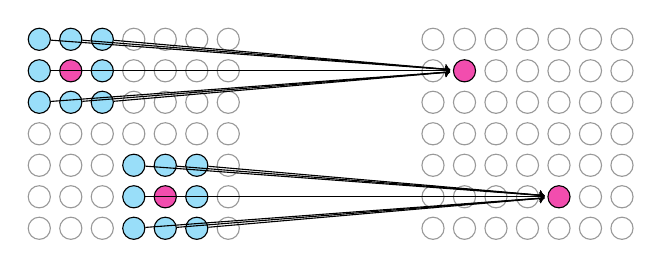
\begin{tikzpicture}
  \tikzstyle{node}=[circle, draw, minimum width=8pt, inner sep=0pt, fill=cyan!40]
  \tikzstyle{gray}=[fill=white, draw=black!40]
  \tikzstyle{root}=[fill=magenta!70]
  \tikzstyle{edge}=[->, shorten >= 1pt]

  \node[node]       (a00) at (0,   0)    {};
  \node[node]       (a10) at (0.4, 0)    {};
  \node[node]       (a20) at (0.8, 0)    {};
  \node[node, gray] (a30) at (1.2, 0)    {};
  \node[node, gray] (a40) at (1.6, 0)    {};
  \node[node, gray] (a50) at (2,   0)    {};
  \node[node, gray] (a60) at (2.4, 0)    {};
  \node[node]       (a01) at (0,   -0.4) {};
  \node[node, root] (a11) at (0.4, -0.4) {};
  \node[node]       (a21) at (0.8, -0.4) {};
  \node[node, gray] (a31) at (1.2, -0.4) {};
  \node[node, gray] (a41) at (1.6, -0.4) {};
  \node[node, gray] (a51) at (2,   -0.4) {};
  \node[node, gray] (a61) at (2.4, -0.4) {};
  \node[node]       (a02) at (0,   -0.8) {};
  \node[node]       (a12) at (0.4, -0.8) {};
  \node[node]       (a22) at (0.8, -0.8) {};
  \node[node, gray] (a32) at (1.2, -0.8) {};
  \node[node, gray] (a42) at (1.6, -0.8) {};
  \node[node, gray] (a52) at (2,   -0.8) {};
  \node[node, gray] (a62) at (2.4, -0.8) {};
  \node[node, gray] (a03) at (0,   -1.2) {};
  \node[node, gray] (a13) at (0.4, -1.2) {};
  \node[node, gray] (a23) at (0.8, -1.2) {};
  \node[node, gray] (a33) at (1.2, -1.2) {};
  \node[node, gray] (a43) at (1.6, -1.2) {};
  \node[node, gray] (a53) at (2,   -1.2) {};
  \node[node, gray] (a63) at (2.4, -1.2) {};
  \node[node, gray] (a04) at (0,   -1.6) {};
  \node[node, gray] (a14) at (0.4, -1.6) {};
  \node[node, gray] (a24) at (0.8, -1.6) {};
  \node[node]       (a34) at (1.2, -1.6) {};
  \node[node]       (a44) at (1.6, -1.6) {};
  \node[node]       (a54) at (2,   -1.6) {};
  \node[node, gray] (a64) at (2.4, -1.6) {};
  \node[node, gray] (a05) at (0,   -2)   {};
  \node[node, gray] (a15) at (0.4, -2)   {};
  \node[node, gray] (a25) at (0.8, -2)   {};
  \node[node]       (a35) at (1.2, -2)   {};
  \node[node, root] (a45) at (1.6, -2)   {};
  \node[node]       (a55) at (2,   -2)   {};
  \node[node, gray] (a65) at (2.4, -2)   {};
  \node[node, gray] (a06) at (0,   -2.4) {};
  \node[node, gray] (a16) at (0.4, -2.4) {};
  \node[node, gray] (a26) at (0.8, -2.4) {};
  \node[node]       (a36) at (1.2, -2.4) {};
  \node[node]       (a46) at (1.6, -2.4) {};
  \node[node]       (a56) at (2,   -2.4) {};
  \node[node, gray] (a66) at (2.4, -2.4) {};

  \node[node, gray] (b00) at (5,   0)    {};
  \node[node, gray] (b10) at (5.4, 0)    {};
  \node[node, gray] (b20) at (5.8, 0)    {};
  \node[node, gray] (b30) at (6.2, 0)    {};
  \node[node, gray] (b40) at (6.6, 0)    {};
  \node[node, gray] (b50) at (7,   0)    {};
  \node[node, gray] (b60) at (7.4, 0)    {};
  \node[node, gray] (b01) at (5,   -0.4) {};
  \node[node, root] (b11) at (5.4, -0.4) {};
  \node[node, gray] (b21) at (5.8, -0.4) {};
  \node[node, gray] (b31) at (6.2, -0.4) {};
  \node[node, gray] (b41) at (6.6, -0.4) {};
  \node[node, gray] (b51) at (7,   -0.4) {};
  \node[node, gray] (b61) at (7.4, -0.4) {};
  \node[node, gray] (b02) at (5,   -0.8) {};
  \node[node, gray] (b12) at (5.4, -0.8) {};
  \node[node, gray] (b22) at (5.8, -0.8) {};
  \node[node, gray] (b32) at (6.2, -0.8) {};
  \node[node, gray] (b42) at (6.6, -0.8) {};
  \node[node, gray] (b52) at (7,   -0.8) {};
  \node[node, gray] (b62) at (7.4, -0.8) {};
  \node[node, gray] (b03) at (5,   -1.2) {};
  \node[node, gray] (b13) at (5.4, -1.2) {};
  \node[node, gray] (b23) at (5.8, -1.2) {};
  \node[node, gray] (b33) at (6.2, -1.2) {};
  \node[node, gray] (b43) at (6.6, -1.2) {};
  \node[node, gray] (b53) at (7,   -1.2) {};
  \node[node, gray] (b63) at (7.4, -1.2) {};
  \node[node, gray] (b04) at (5,   -1.6) {};
  \node[node, gray] (b14) at (5.4, -1.6) {};
  \node[node, gray] (b24) at (5.8, -1.6) {};
  \node[node, gray] (b34) at (6.2, -1.6) {};
  \node[node, gray] (b44) at (6.6, -1.6) {};
  \node[node, gray] (b54) at (7,   -1.6) {};
  \node[node, gray] (b64) at (7.4, -1.6) {};
  \node[node, gray] (b05) at (5,   -2)   {};
  \node[node, gray] (b15) at (5.4, -2)   {};
  \node[node, gray] (b25) at (5.8, -2)   {};
  \node[node, gray] (b35) at (6.2, -2)   {};
  \node[node, root] (b45) at (6.6, -2)   {};
  \node[node, gray] (b55) at (7,   -2)   {};
  \node[node, gray] (b65) at (7.4, -2)   {};
  \node[node, gray] (b06) at (5,   -2.4) {};
  \node[node, gray] (b16) at (5.4, -2.4) {};
  \node[node, gray] (b26) at (5.8, -2.4) {};
  \node[node, gray] (b36) at (6.2, -2.4) {};
  \node[node, gray] (b46) at (6.6, -2.4) {};
  \node[node, gray] (b56) at (7,   -2.4) {};
  \node[node, gray] (b66) at (7.4, -2.4) {};

  \path[edge] (a00) edge (b11);
  \path[edge] (a10) edge (b11);
  \path[edge] (a20) edge (b11);
  \path[edge] (a01) edge (b11);
  \path[edge] (a11) edge (b11);
  \path[edge] (a21) edge (b11);
  \path[edge] (a02) edge (b11);
  \path[edge] (a12) edge (b11);
  \path[edge] (a22) edge (b11);

  \path[edge] (a34) edge (b45);
  \path[edge] (a44) edge (b45);
  \path[edge] (a54) edge (b45);
  \path[edge] (a35) edge (b45);
  \path[edge] (a45) edge (b45);
  \path[edge] (a55) edge (b45);
  \path[edge] (a36) edge (b45);
  \path[edge] (a46) edge (b45);
  \path[edge] (a56) edge (b45);
\end{tikzpicture}
\caption[Faltung innerhalb eines \glspl{CNN}]{Illustration der Neuronenverbindungen in einem \gls{CNN} bei einer Filtergröße von $3 \times 3$, hier am Beispiel von zwei Neuronen (rot).
Der Wert eines Neurons berechnet sich aus allen Neuronen innerhalb eines Receptive-Fields um das Neuron der vorherigen Schicht (blau).}
\label{fig:cnn}
\end{figure}
